\documentclass[11pt, twocolumn]{article}
\usepackage{graphicx}
\usepackage{enumitem,kantlipsum}
% \usepackage[LGRgreek]{mathastext}
\usepackage[document]{ragged2e}
\usepackage{hyperref}
\usepackage{geometry}
\usepackage{titlesec}
\usepackage{floatrow}
\usepackage{caption}
\titlespacing{\title}{0pt}{\parskip}{-\parskip}
\usepackage{sectsty}
\sectionfont{\Large}
\newgeometry{left=15mm, right=15mm , top=20mm , bottom =20mm}

\setlength{\parindent}{0em}
\title{
Impact of World Events on Tech Stocks \\
DS203 Course Project
}
\author{Rohan Nafde 210070068\\
Sajal Deolikar 210070071\\
Varad Deshpande 21d070024}
\date{}
\begin{document}

\maketitle

\begin{justify}

\section*{\huge Introduction}\label{sec:intro}

\vspace{-5pt}

Stocks signify ownership of a part of a corporation, its assets and its earnings.
Naturally, their value reflects how valuable the corporation is perceived to be by the investors.
Major world events impact stocks as they change people's thoughts and expectations, thus changing 
the perceived value.
\vspace{1em}

In this project, we take a deeper dive into the impact of world events on the valuation of the stocks
of major tech companies. After exploratory data analysis and identifying trends, we attempt to fit a 
model to predict the future impacts of such occurrences.

\begin{figure}[h]
  \centering
  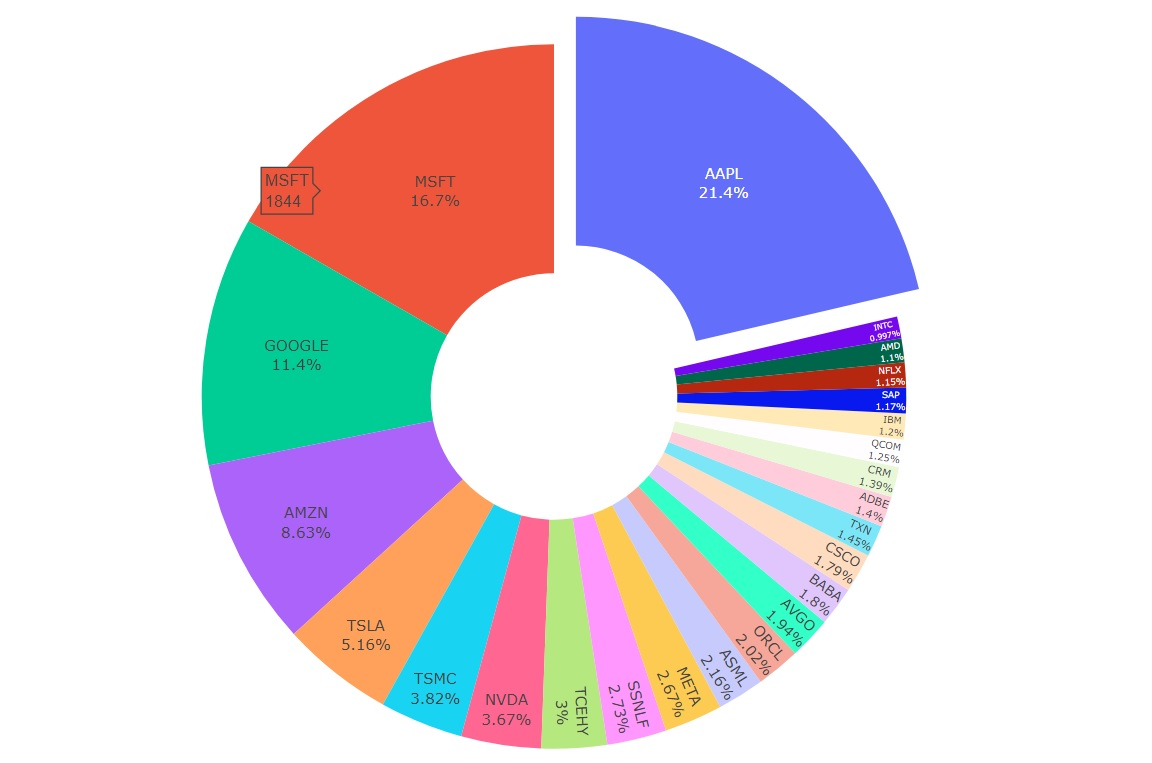
\includegraphics[scale=0.4]{figs/pie.jpg}
  \caption*{Market Capital}
\end{figure}

\section{\huge EDA}\label{sec:eda}

\vspace{-5pt}

\subsection{Data Acquisition}
Our main goal was to get the data of stock prices of big tech companies (open, high, low, close) for each day for the years 2006-2022. We searched online and found a dataset of the top 100 big tech companies for the above years, and we downloaded that. Later we learned that this data was downloaded using the "yfinance" library of python, which we used to download further desired data.\vspace{-5pt}
\subsection{Cleaning the Data} 
he data was pretty clean, and we removed files that had many NA cells in them. Rest all were cleaned by basic EDA techniques taught (replacing blank spaces with NA, etc.)
\vspace{-5pt}
\subsection{Preliminary Observations}
After we plotted candlestick plots for all data, we quickly discovered the fluctuations in stock prices during certain events. The aggregate plot reveals a major dip in stock prices in the years 2008 (recession) and 2020 (Covid). But then there were certain companies that performed well nevertheless (like Tesla and Zoom in Covid). All these interesting observations have been further summarised below.


\section{\huge World Events and their Impact}
\vspace{-5pt}

\subsection{Great Recession (2008)}
The combination of widspread failures in financial regulation, excessive risk and lack of understanding of the financial system led to the housing bubble burst from 2007-2009.
The International Monetary Fund concluded that it was the most severe economic meltdown since the Great Depression.
\vspace{1em}


By plotting the market value taking 100 prominent tech companies into account, we can see that the market dropped by over
40\% during the recession.

\vspace{-5pt}
\begin{figure}[h]
  \centering
  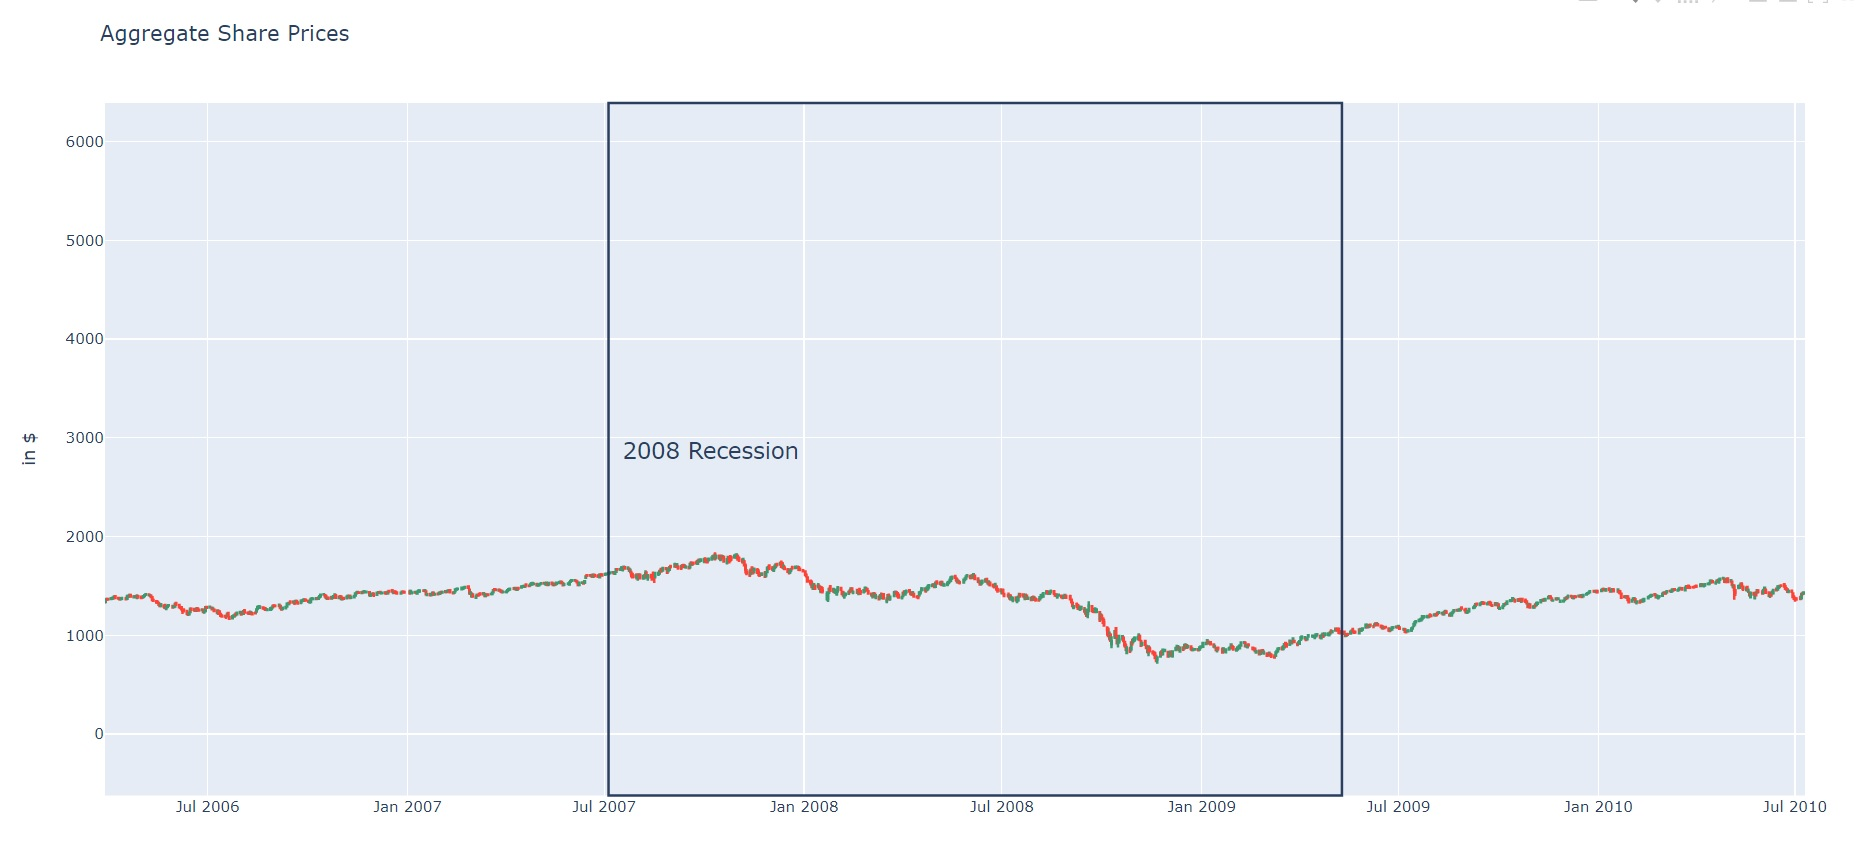
\includegraphics[scale=0.24]{figs/rec.jpg}
  \caption*{Market from 2006-2010}
\end{figure}

\subsection{Covid-19 Pandemic (2019-2021)}
The COVID-19 pandemic has resulted in over 4.3 million confirmed cases and over 290,000 deaths globally.
The widespread panic, uncertainty, and poor government decisions during the Covid pandemic caused the stock market to crash.
Many small-scale businesses had to shut down as a result of the lockdowns imposed around the world.
\vspace{1em}


However, some companies did flourish during the pandemic. Zoom's share prices skyrocketed to ten times their original value due to its widespread usage in CoViD.
Tesla's share price also increased eightfold. Some companies like NVidia released their latest and greatest GPUs (RTX) which people bought to play video games to
kill time (not seeing the costs). This made their share price also increase. The same goes with AMD (who released their next gen Ryzen CPUs) and Intel.

\vspace{-5pt}
\begin{figure}[h]
  \centering
  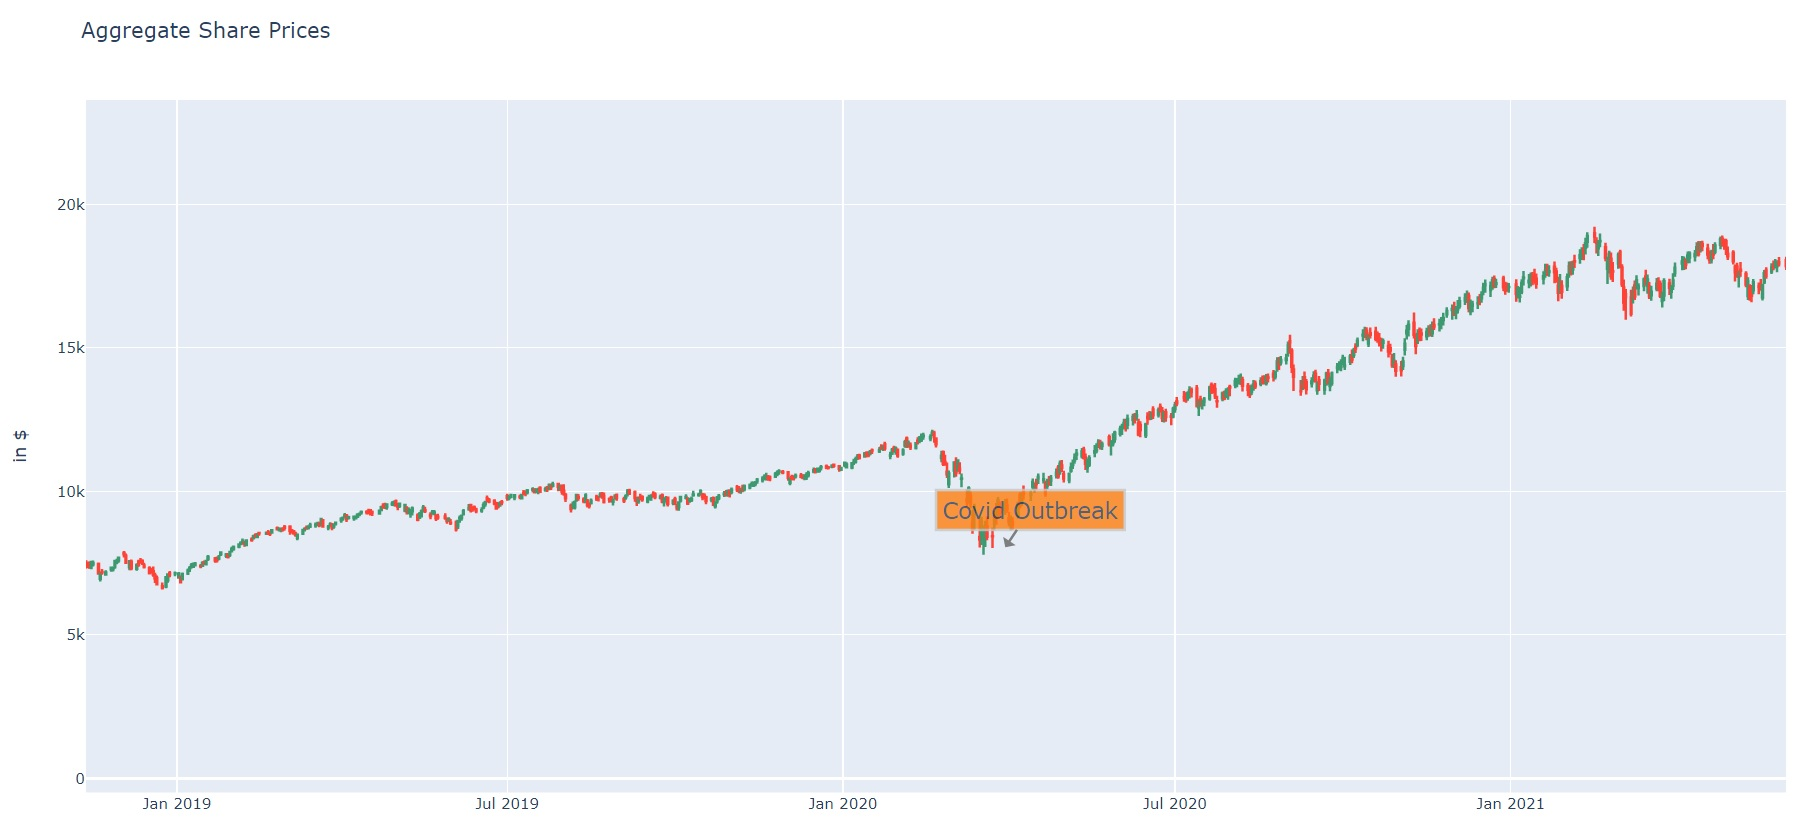
\includegraphics[scale=0.24]{figs/covid.jpg}
  \caption*{Impact of the Covid Pandemic}
\end{figure}


\subsection{U.S.-China Trade War (2018-present)}
In January 2018, the Trump administration began setting tariffs and other trade barriers on China to force it to make changes to longstanding unfair trade practices and intellectual property theft, according to the U.S. \vspace{1em}


In response to US trade measures, the Chinese government accused the Trump administration of engaging in nationalist protectionism and took retaliatory action. A series of tariffs, import restrictions, agreements and name-calling followed. By the end of the Trump presidency, the trade war was characterized as a failure. His successor, Joe Biden, has kept the tariffs.
\vspace{-5pt}

\subsection{Brexit (June 2016)}
The stock market suffered its worst drop in 10 months as shock over the United Kingdom voters' move to exit the European Union sent markets in a tailspin. Amid uncertainty regarding the
impact of Brexit, stock prices fell by over 3\% and even by 8\% in some markets.
\vspace{1em}


Panick ensued because there was a false sense of security that the British voters would vote to stay in the EU. Analysts concluded that investors overreacted, as in a low-growth environment, uncertainty or increased concerns really do create tremendous volatility.

\vspace{-5pt}

\begin{figure}[h]
  \centering
  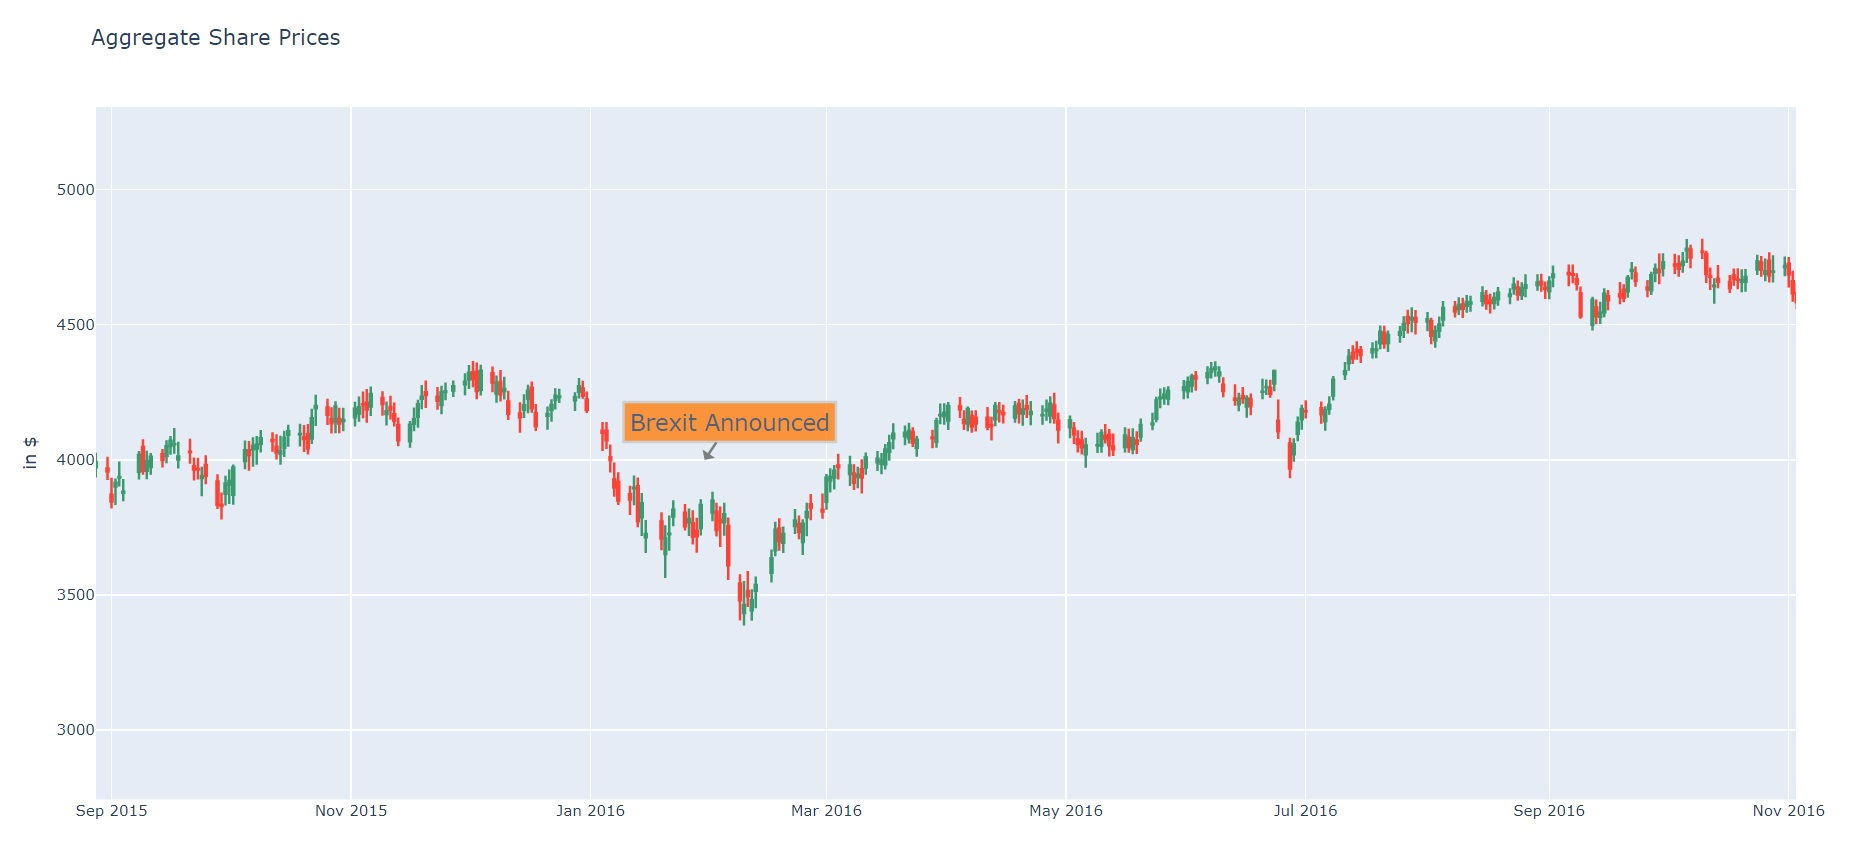
\includegraphics[scale=0.23]{figs/brexit.jpg}
  \caption*{Impact of Brexit}
\end{figure}

\subsection{Russia-Ukraine War (2014-present)}
Following Ukraine's Revolution of Dignity, Russia annexed Crimea from Ukraine in 2014 and supported pro-Russian separatists in Donbas against Ukrainian government forces.
Fighting for the first eight years of the conflict included naval incidents, cyberwarfare, and heightened political tensions.
\vspace{1em}


In February 2022, the conflict saw a major escalation as Russia launched a full-scale invasion of Ukraine. The ongoing full-scale war has resulted in a major refugee crisis and tens of thousands of deaths. It caused the price of energy, commodities and metals, which Russia is one of the largest producers and exporters of.

\vspace{-5pt}



\section{\huge Interesting Trends}
\vspace{-5pt}

\begin{figure}[h]
  \centering
  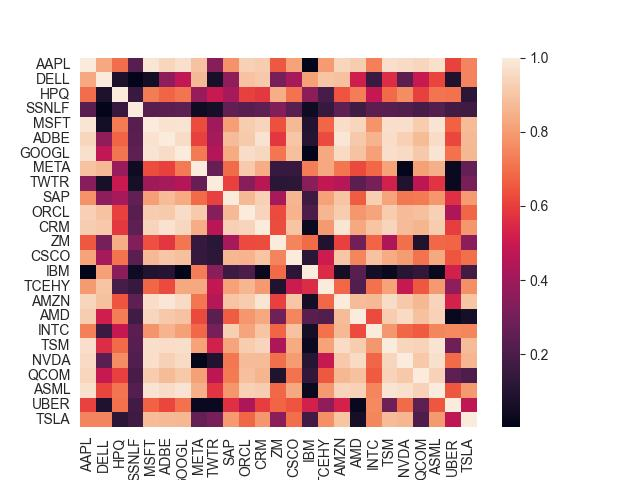
\includegraphics[scale=0.6]{figs/heat_map.jpeg}
  \caption*{Correlation between stock prices}
\end{figure}


\subsection{AMD's fall and rebirth}
AMD is one of the oldest designers of large scale microprocessors and its story is filled with successes, errors and a close shave with ruin. In the early days, what Intel designed, AMD simply tried to make better. The poor decisions, lawsuits and inability to design a competitive product nearly drove AMD to bankruptcy in 2014.
\vspace{1em}


However, the change of leadership and strategy lead to the development of the Zen architecture in 2017, which proved to be a game-changer for AMD. Finally, AMD's chips were competitive causing a large increse in profits. Today, AMD competes with both Intel and NVIDIA and their chips are used in Tesla cars, gaming consoles, laptops, PCs etc. and we can see the correlation in their stock prices in the correlation matrix.
\vspace{-5pt}

\begin{figure}[h]
  \centering
  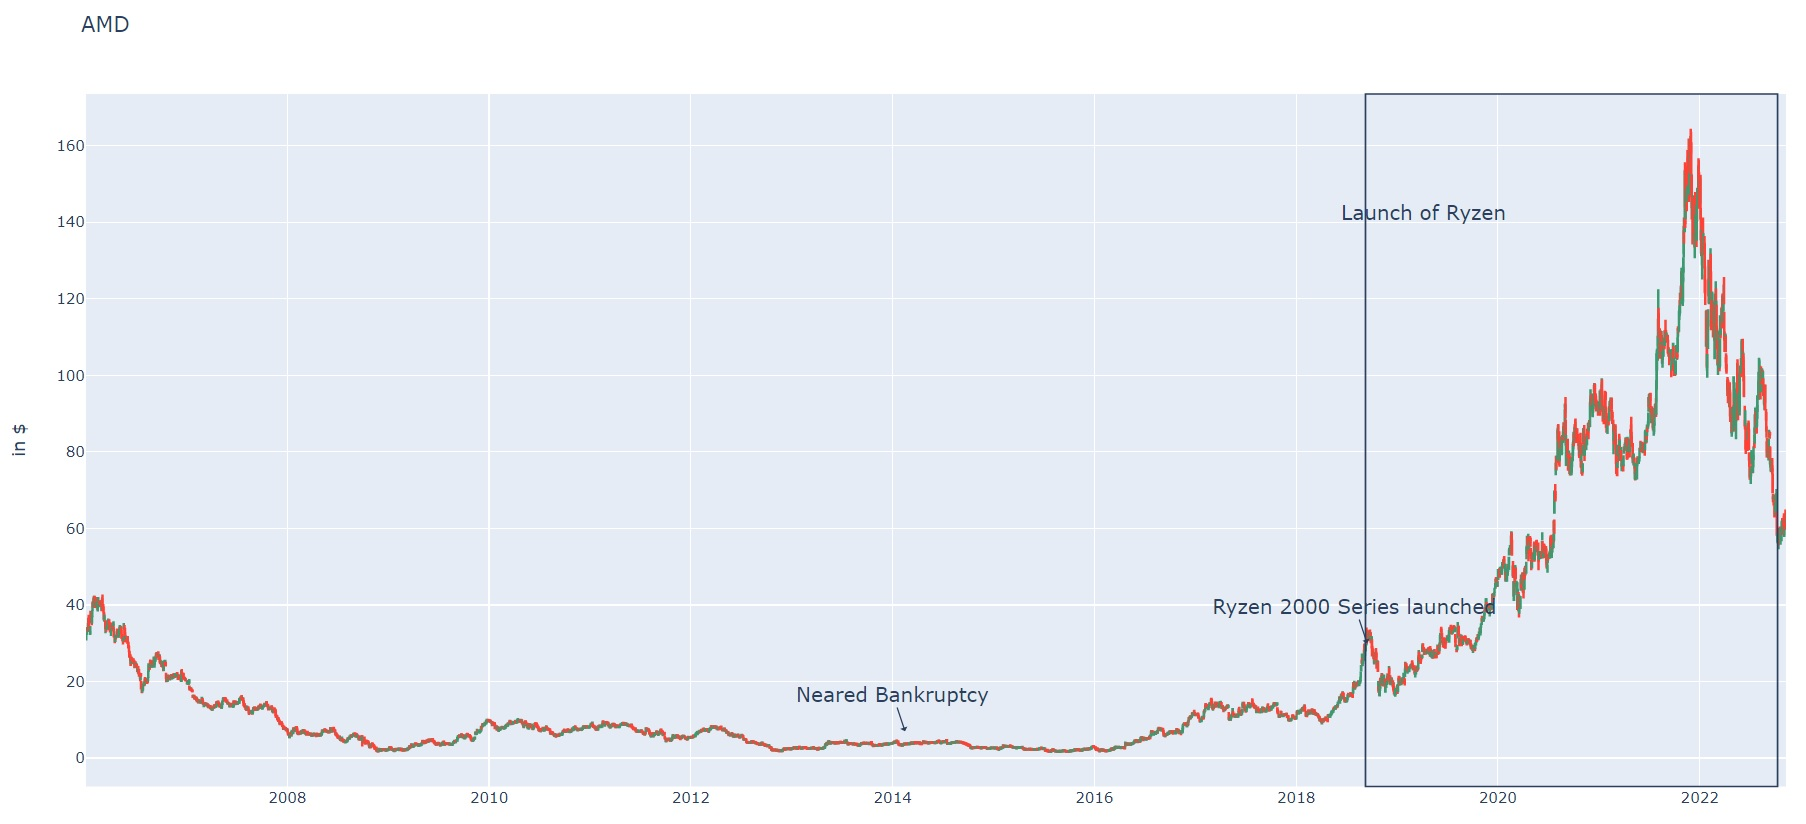
\includegraphics[scale=0.24]{figs/amd.jpg}
  \caption*{AMD's stock price}
\end{figure}

\subsection{iPhone, iPad and M1}
The original iPhone release in June 2007 heralded a new era of tech and defined what smartphones are today. Despite the
doubts surrounding, it at the time it is still Apple's most successful product line.
\vspace{1em}


The iPad announcement in Jan 2010 initially had mixed reception by the media, but it was well-received for its software and was recognized as one of the most-influential inventions.
\vspace{1em}


Interestingly, Apple's stocks were not affected much by the iPhone annoucement, but increased significantly due to the iPad. This may show the difference in investors' opinion and
confidence in Apple before and after the iPhone. Apple's stock prices have sky-rocketed ever since, more so with the introduction of M1 in 2020.
\vspace{-5pt}

\begin{figure}[h]
  \centering
  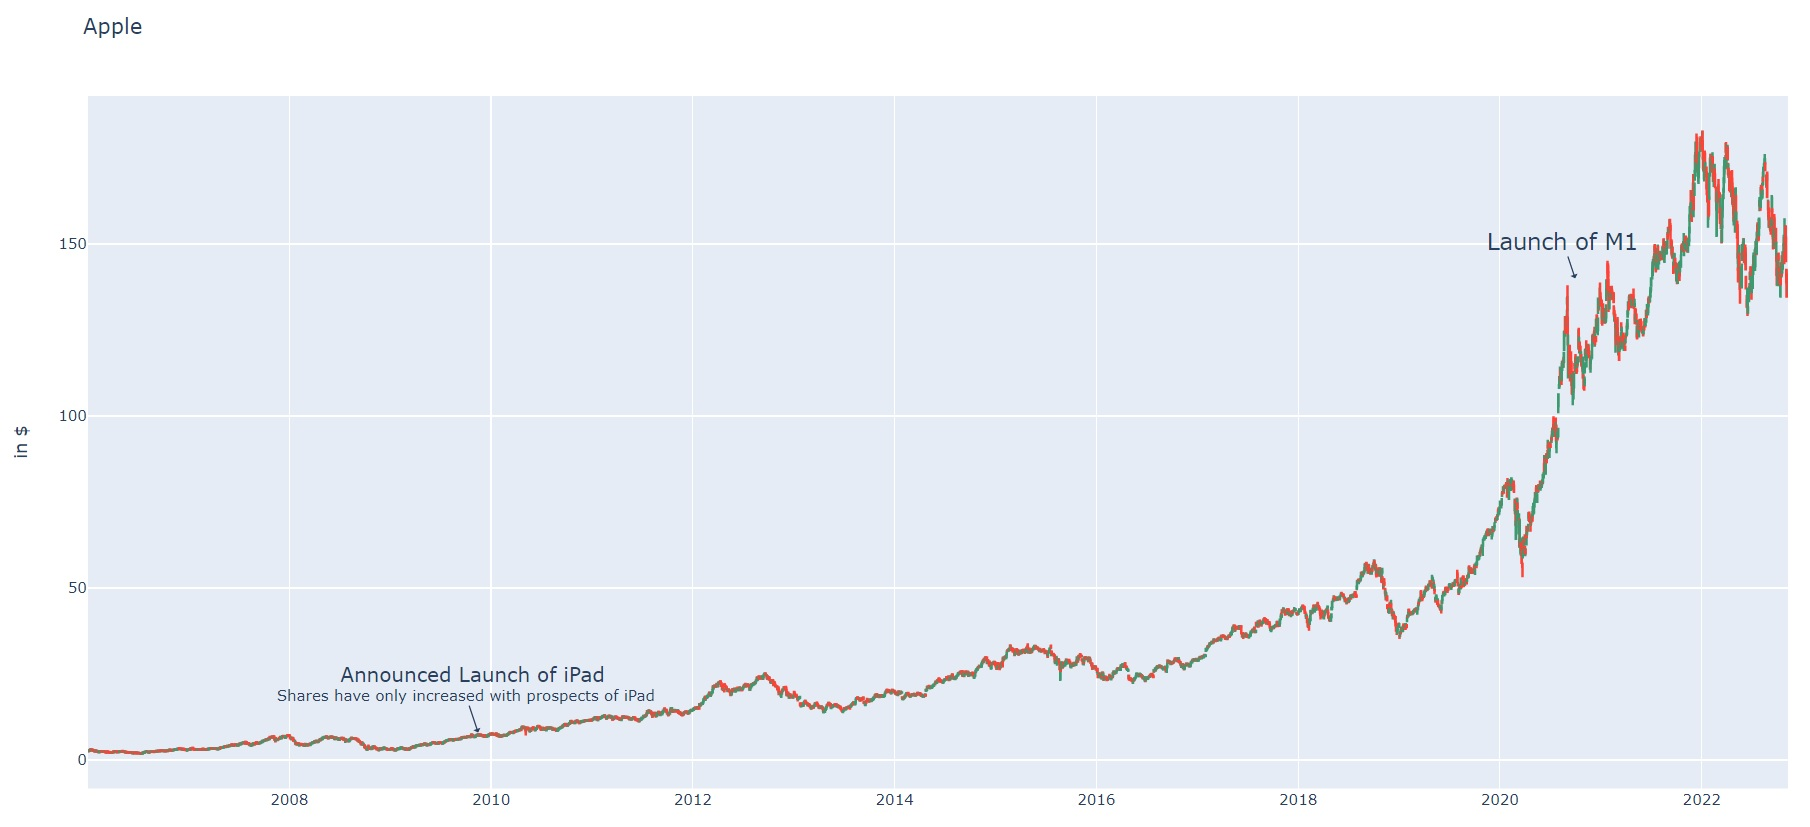
\includegraphics[scale=0.24]{figs/apple.jpg}
  \caption*{Apple's stock price}
\end{figure}

\subsection{DELL vs. HP}
DELL and HP are two of the world's largest electronic hardware companies that make a vairety of products including laptops, desktops, printers, monitors, TVs etc.
Given their large sizes and large overlap of target markets, we can expect a negative correlation in their stock prices.
\vspace{1em}


This means that when investors are confident of one company, they lose confidence in the other. From the stock price graphs and the correlation matrix we can see that this is indeed the case.
\vspace{-5pt}

\begin{figure}[h]
  \centering
  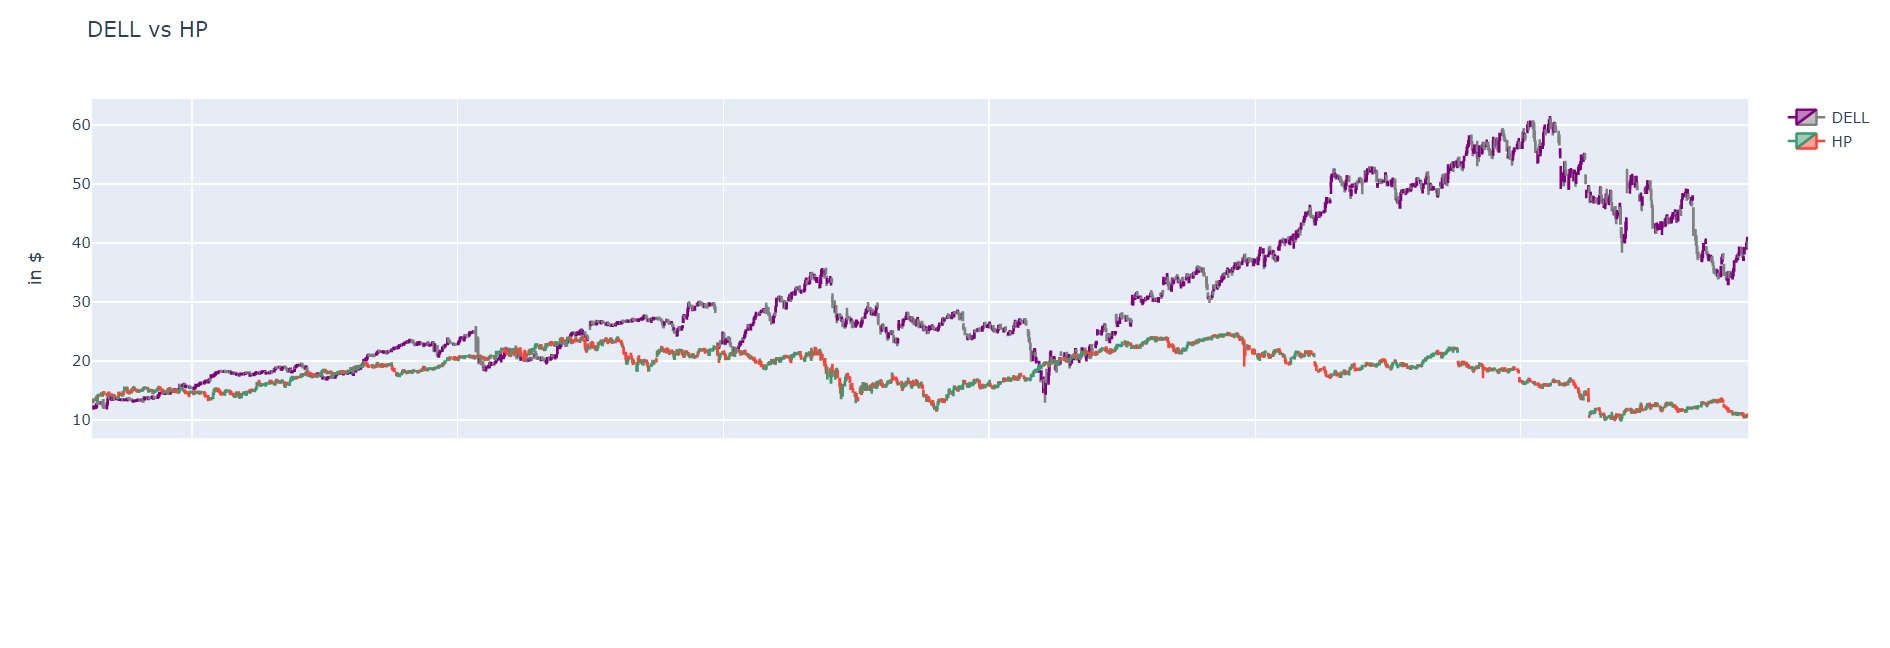
\includegraphics[scale=0.24]{figs/hpdell.jpg}
  \caption*{HP vs. DELL}
\end{figure}

\subsection{Alphabet and Microsoft}
Alphabet consists of various companies like Google, Nest, Calico and X development, each with different goals is one of the most valuable companies in the world. Microsoft,
a name heard by practically everyone, is the software and electronics company that is responsible for Windows.
\vspace{1em}

\begin{figure}[h]
  \centering
  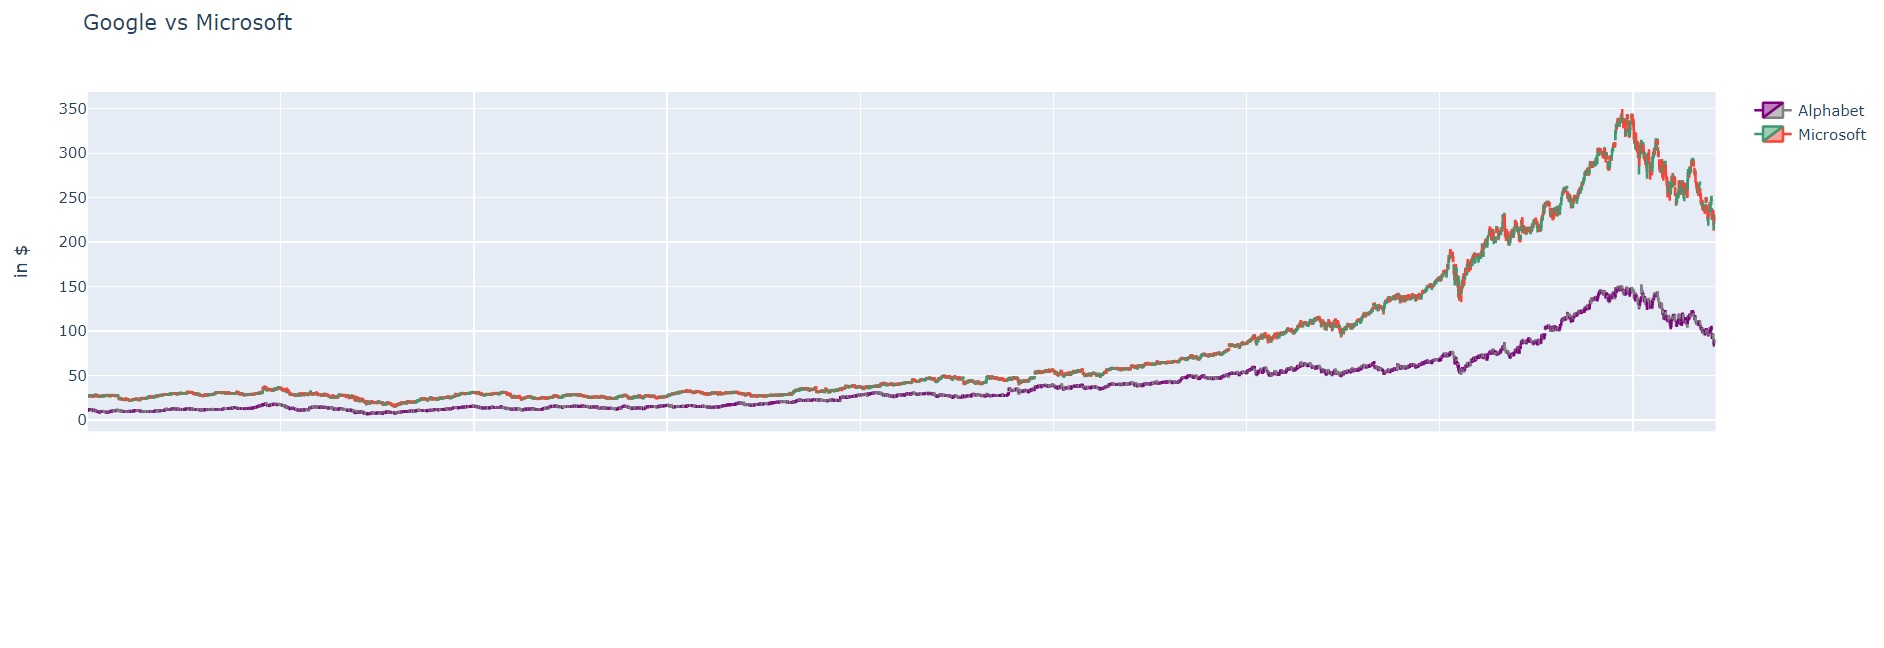
\includegraphics[scale=0.24]{figs/msgoogle.jpg}
  \caption*{Alphabet vs. Microsoft}
\end{figure}

Their stock prices have a positive correlation as seen in the correlation heatmap and their stock price plots. This is counter-intuitive and may point to the fact that they are not
direct competitors in most spaces except areas like cloud services and search engines.
\vspace{-5pt}

\subsection{Rise of Zoom (2020)}
Before the Covid pandemic, Zoom was a video conferencing tool like any other, mainly used by employees for conferences and communication. However, once lockdowns were enforced, there was a surge in the use of video conferencing platforms and Zoom was able to rise above the rest.
\vspace{1em}


Zoom was successful because of its plethora of free features, easy accessibility and capabilities to host meetings with a large number of attendees. In 2020, Zoom's revenue increased by over 169\%
and it peaked at over 300 million daily meeting participants (30 fold of 2019). Despite the crashing market, Zoom was did extremely well during the pandemic. As expected, Zoom's stock price has started droppiing after lockdowns were removed around the world.
\vspace{-5pt}

\begin{figure}[h]
  \centering
  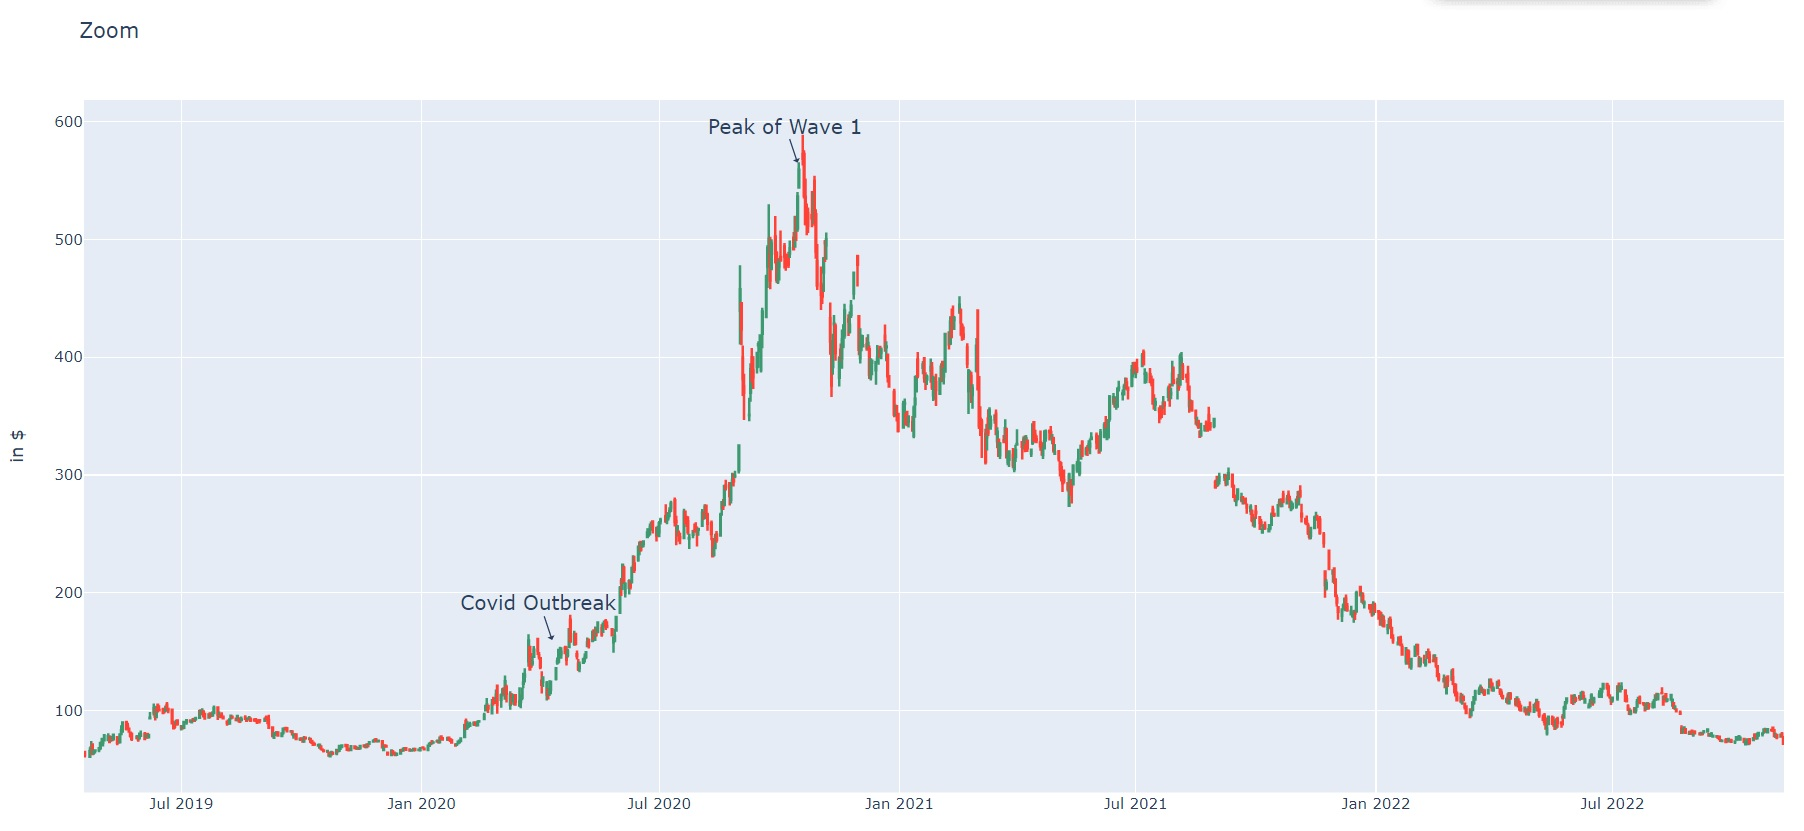
\includegraphics[scale=0.25]{figs/zoom.jpg}
  \caption*{Zoom's stock price}
\end{figure}

\subsection{Telsa powers through Covid}
Tesla, the renewable energy and electric car company lead by Elon Musk, had a remarkable year in 2020 with its stock prices increasing by almost 8x. While Covid hit other car manufacturers hard,
Tesla grew thanks to the lanuch of the Model Y, commencement of production in its Chinese factory, better software and battery advancements.
\vspace{1em}


Despite the controversial statements made by Musk about the Covid pandemic and employees' woes about the company not reacting to Covid, Tesla's position continued to strengthen.
Moreover, the rise was compounded due to Telsa's entry into the S\&P500.
\vspace{-5pt}

\begin{figure}[h]
  \centering
  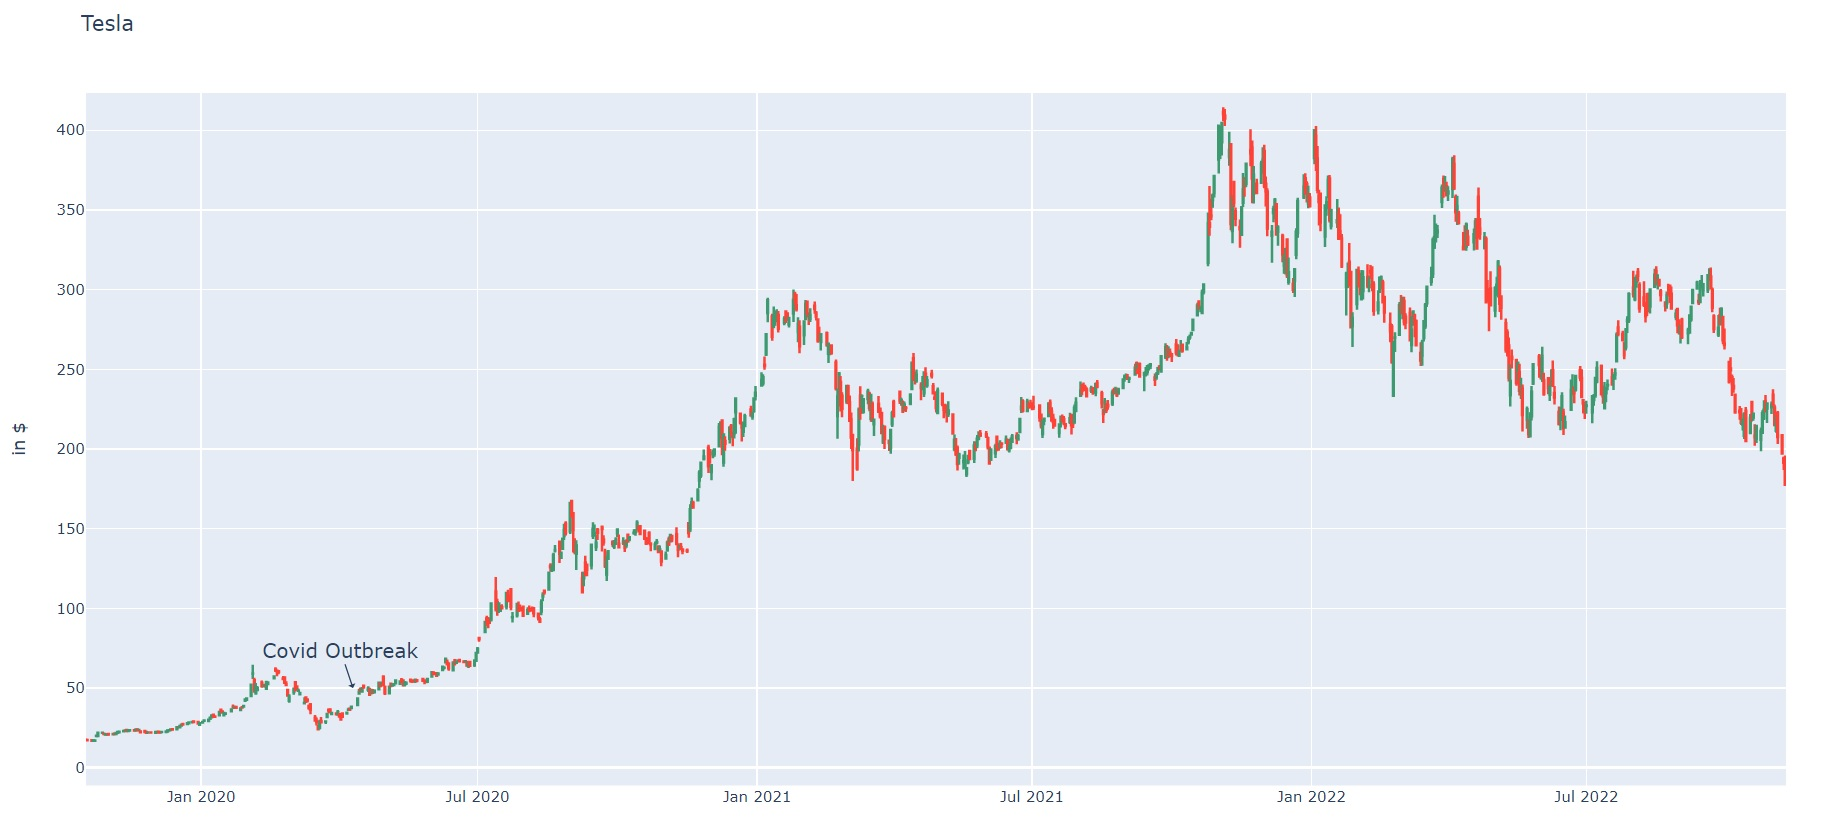
\includegraphics[scale=0.24]{figs/tesla.jpg}
  \caption*{Tesla's stock price}
\end{figure}


\subsection{Musk buys Twitter (2022)}
The largest recent event in the tech world was Elon Musk's takeover of Twitter by a total buyout of 45 billion USD.
Musk privatized Twitter, fired many top officials and cut down the workforce by over half in a very short period of time.
\vspace{1em}


Such uncertainty
\vspace{-5pt}




\section{\huge Modelling stock price fluctuations}
\vspace{-5pt}
Write about which model we're trying to fit and why. How did we do it? What are our conclusions?



\section{\huge Conclusions}

\vspace{-5pt}



\end{justify}
\end{document}
